\documentclass[notitlepage]{fhnwreport}

\usepackage[T1]{fontenc}
\usepackage[english]{babel}
\usepackage{csquotes}
\usepackage{lmodern}
\usepackage{kpfonts}
\usepackage{hyperref}
\usepackage[backend=bibtex,bibstyle=numeric,sorting=nyt]{biblatex}
\usepackage[para,online,flushleft]{threeparttable}
\usepackage{booktabs}
\usepackage{lipsum}
\usepackage{float}
\usepackage{multicol}
\usepackage{titling}
% Post title
\newcommand{\subtitle}[1]{%
  \posttitle{%
    \par\end{center}
    \begin{center}\large#1\end{center}
    \vskip0.5em}%
}
% Move title up to top of page
\setlength{\droptitle}{-10em}

\addbibresource{bibliography.bib}

\title{Treasure Planet}
\subtitle{Archplot Structure Analysis}
\author{Alex Murray}

\begin{document}
\maketitle

\begin{figure*}[th!]
    \centering
    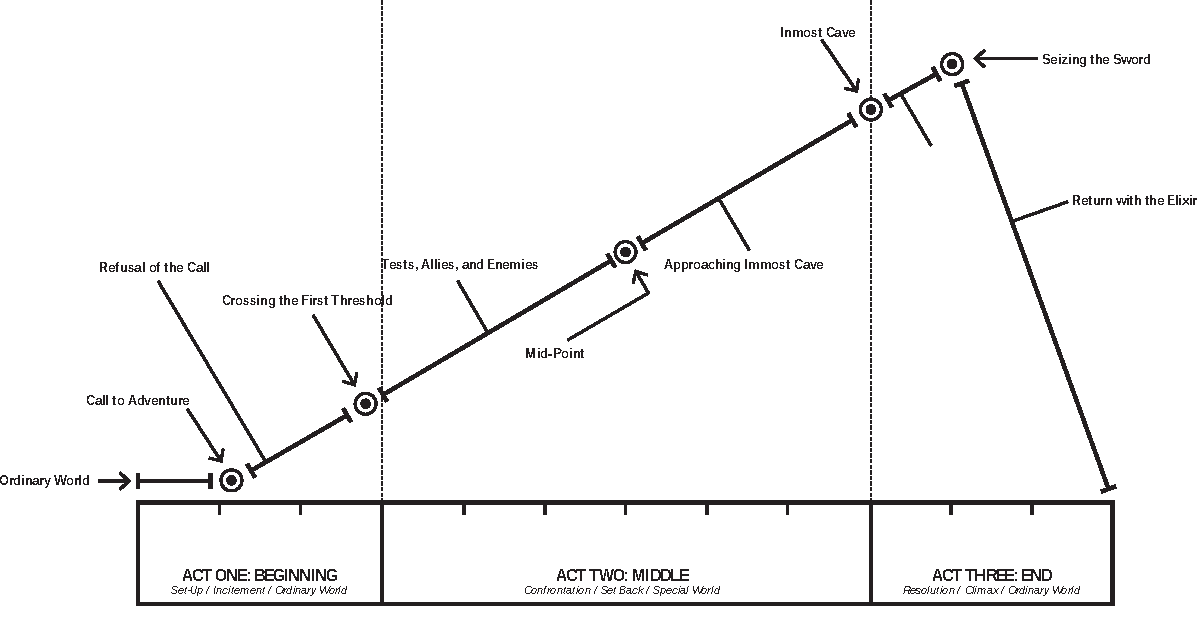
\includegraphics[width=\linewidth]{archplot.pdf}
    \caption{Structure of \textit{The Hero's Journey} in function of time.}
    \label{fig:archplot}
\end{figure*}

\begin{multicols}{2}

\section*{Treasure Planet}

In  this  report, we will break down the plot structure of the movie  Treasure
Planet\cite{ref:treasure-planet}.  It  follows  a  well-known  plot  structure
\textit{The  Hero's  Journey}\cite{ref:heros-journey}  which  is  depicted  in
figure \ref{fig:archplot}.

\subsection*{Ordinary World}

As  a child, the main character \textit{Jim Hawkins} was enchanted by  stories
of  a  pirate  named  \textit{Captain  Flint} who mysteriously appeared out of
nowhere to raid freight ships and soon  after  vanished.  Legend says that the
loot he stole  was  stashed  on  an  unknown  planet  called  \textit{Treasure
Planet}. It  is  clear that Jim was completely captivated by the adventures of
spacers  and  was  in  a  loving  and tender  relatoinship  with  his  mother.

12 years later, we are re-introduced to Jim  as  somewhat  of  a misunderstood
teenage rebel  who  clearly  doesn't  want  his  actions  to  hurt  anyone  --
especially  his  mother  --  but doesn't understand how to or maybe feels it's
pointless to communicate that  to  her. He knows he keeps letting her down but
has  resigned  himself  to  the idea that he has no future, so why  should  he
worry? He reluctantly helps his mother \textit{Sarah} run the  family's Benbow
Inn and derives  amusement  from  skysurfing  on  a  rocket-powered sailboard.

\subsection*{Call to Adventure}

One day, a spaceship crash lands near the Benbow Inn. Jim runs out to help the
dying  pilot,  who  hands  him a metal sphere and tells him to beware  of  the
cyborg. Shortly after,  a  gang  of pirates show up and burn down the Inn. Jim
and  his  mother  escape  along  with  a dog-like friend  \textit{Dr.  Delbert
Doppler}, who offers them shelter at his study.

\subsection*{Refusal of the Call}

At Doppler's study,  they discover that the sphere Jim was given is actually a
holographic  projector,  showing  a star map that leads  to  the  location  of
Treasure Planet. Jim's  mother,  being  a  mother, is of course opposed to the
idea of Jim and Doppler  going  on  a  dangerous  adventure for something that
might  not  even  exist  --  Treasure  Planet  is  just  a  legend after  all.

Jim  feels  like the Inn burning down was his fault and  he  wants  to  redeem
himself  by  going  on  this  adventure, finding the treasure, and  funding  a
rebuild of the Inn.

Sarah,  the mother, eventually agrees and Jim and Dr. Doppler commision a ship
called  the  \textit{RLS  Legacy}  on  a  mission  to  find  Treasure  Planet.

\subsection*{Crossing the First Threshold}

Jim  and  Doppler  are  introduced  to the captain, \textit{Captain Amelia}, a
cat-like  English  woman,  along  with her stone-skinned and disciplined first
mate \textit{Mr. Arrow}.  Jim  is  further  introduced  to  the  ship's  cook,
\textit{John Silver}, who turns out to be a cyborg. Jim  suspects  this is the
cyborg he was warned about.

The ship sets sail and they are off to an adventure!

\subsection*{Tests, Allies, and Enemies}

There are many incidences  that occur on the ship during their journey through
space.

It is revealed that Jim's father abandoned him at  an  early  age. Silver, the
cyborg Jim is  suspicious  of, ends up growing closer and fills the father-son
role Jim never had as a child. He's tough on Jim but also ends up teaching him
a lot of skills.

It also becomes clear that the crew is  secretly being led by Silver, and they
are planning a mutiny.

The ship encounters a supernova which turns into a black  hole. This moment in
the movie tests who is allied with whom.  Among  the chaos, Jim ends up saving
Silver from fallling into the  black  hole,  thus  saving his life. Arrow, the
captain's first mate, ends up  falling  into  the  black hole as a result of a
shady spider-like crew member cutting his lifeline on purpose.

\subsection*{Mid-Point}

Jim overhears Silver's real plan and learns that the crew are pirates. As they
reach Treasure planet, mutiny erupts. Jim, Dr. Doppler, and Amelia abandon the
ship  along  with  what  they at the time believe to be the map. An  important
moment  here  is  when Silver has the opportunity to shoot and kill  Jim,  but
can't  do it.They crash land on the surface of Treasure Planet  in  an  escape
ship and seak cover in a hidout.

\subsection*{Approaching Inmost Cave}

While exploring Treasure Planet's  forests,  they  meet  B.E.N.,  an abandoned
robot,  who  lost his primary memory circuits. The robot invites them into its
shelter.

It turns out the map they thought they had was in  fact  a  fake copy, and the
real map was still abord the ship. The pirates, though, still believe that Jim
is in possession of the map.

They  learn  about  the  planet  center  being a gigantic machine filled  with
tunnels. Jim uses this  to  his  advantage to slip by the pirates, who are now
searching for them, and to steal the piarate's escape  ship and go back to the
main ship to retrieve the real map.

He successfully  retrieve  the  map  and  returns to the planet's surface, but
finds   Doppler  and  Amelia  captured  by  the  Silver   and   his   pirates.

\subsection*{Inmost Cave}

Only Jim  knows how to unlock the map, so Silver forces Jim to use the map and
in return agrees to spare their lives. The map leads  them  to  a portal which
can  be  opened to any location in the galaxy. This is how Captain  Flint  was
able to appear out of nowhere and disappear again. They open the portal to the
planet's center and find the treasure of a thousand worlds.

\subsection*{Seizing the Sword}

The planet was  rigged  with  booby traps, which triggered as they entered the
planet's  core.  The  entire  planet is set to blow in just a few minutes  and
begins falling apart.

Jim finds an old ship among the gold and  is  able to start it up. Silver sees
Jim  doing  this  and  decides to try and take the ship for himself. As Silver
confronts Jim, a violent eruption from  the  planet's  core  bumps him off the
ship and leaves him hanging off of a cliff, one which would surely kill him if
he were to  let  go. Silver is left to make a choice: Either he takes the ship
filled  with treasure and leaves Jim to die, or he abandons the ship and saves
Jim's life. He chooses to do the latter.

\subsection*{Final Push}

Jim,  Silver,  Doppler  and  Amelia  have just minutes to escape the exploding
planet. They  do so with the original ship, the RLS Legacy, and fly it through
the portal to safety.

\subsection*{Return with Elixir}

Silver parts ways with Jim, as he doesn't want  to  be arrested and jailed for
the crimes  he  has  committed.  Jim returns with pockets full of treasure and
rebuilds the Inn with his mother.

Sometime later, a party is hosted at the rebuilt Inn, where Doppler and Amelia
are married,  have  children  of  their own, and Jim becomes a military cadet.

\printbibliography

\end{multicols}

\end{document}
